\documentclass[a4paper,12pt]{article}

% --- Pacchetti ---
\usepackage[utf8]{inputenc}
\usepackage[T1]{fontenc}
\usepackage[italian]{babel}
\usepackage{amsmath,amssymb}
\usepackage{graphicx}
\usepackage{booktabs}
\usepackage{siunitx}
\usepackage[margin=2.5cm]{geometry}
\usepackage{hyperref}
\usepackage{fancyhdr}
\usepackage{listings}
\usepackage{xcolor}
\usepackage{float}
\usepackage{mathtools}

% --- Configurazione listing ---
\definecolor{codegreen}{rgb}{0,0.6,0}
\definecolor{codegray}{rgb}{0.5,0.5,0.5}
\definecolor{codepurple}{rgb}{0.58,0,0.82}
\definecolor{backcolour}{rgb}{0.95,0.95,0.92}

\lstdefinestyle{mystyle}{
    backgroundcolor=\color{backcolour},   
    commentstyle=\color{codegreen},
    keywordstyle=\color{magenta},
    numberstyle=\tiny\color{codegray},
    stringstyle=\color{codepurple},
    basicstyle=\ttfamily\footnotesize,
    breakatwhitespace=false,         
    breaklines=true,                 
    captionpos=b,                    
    keepspaces=true,                 
    numbers=left,                    
    numbersep=5pt,                  
    showspaces=false,                
    showstringspaces=false,
    showtabs=false,                  
    tabsize=2
}
\lstset{style=mystyle}

% --- Intestazioni ---
\pagestyle{fancy}
\fancyhf{}
\fancyhead[L]{Progetto MCS - Solutori iterativi per sistemi lineari}
\fancyhead[R]{N. Chines, J. Borgato}
\fancyfoot[C]{\thepage}

% --- Titolo ---
\title{\textbf{Mini Libreria per Sistemi Lineari}\\[5pt]
       \large Metodi iterativi per matrici simmetriche e definite positive}
\author{
    Nicolas Chines (matr. 899536)\\
    Jacopo Borgato (matr. 866305)\\[10pt]
    Corso di Metodi per il Calcolo Scientifico\\
    Università degli Studi di Milano-Bicocca\\
    Anno Accademico 2025-2026
}
\date{\today}

\begin{document}
\maketitle
\thispagestyle{empty}

\begin{abstract}
Il progetto consiste nella realizzazione di una libreria Python per la risoluzione di sistemi lineari con matrice simmetrica e definita positiva (SPD). Sono stati implementati quattro metodi iterativi: Jacobi, Gauss-Seidel, Gradiente (Steepest Descent) e Gradiente Coniugato. Il codice, corredato da un'interfaccia a riga di comando e da una moderna interfaccia utente testuale (TUI) realizzata con la libreria \texttt{Textual}, è stato testato su matrici sparse reali. Le prestazioni sono state confrontate in termini di iterazioni, tempo di esecuzione ed accuratezza per tolleranze comprese tra $10^{-2}$ e $10^{-10}$. In questo resoconto vengono illustrati i fondamenti matematici, le considerazioni sull'aritmetica in virgola mobile, le scelte implementative, i risultati sperimentali e le conclusioni tratte dall'analisi.
\end{abstract}

\vspace{1cm}
\noindent\textbf{Repository GitHub}: \url{https://github.com/deltanicolas/Progetto_Metodi_del_Calcolo_Scientifico_Unimib} \\
\noindent\textbf{Autori}: Nicolas Chines (deltanicolas), Jacopo Borgato

\newpage
\tableofcontents
\newpage

% ==============================================================================
\section{Introduzione}
% ==============================================================================
La risoluzione di sistemi lineari di grandi dimensioni è un problema centrale nel calcolo scientifico. Quando la matrice dei coefficienti è simmetrica e definita positiva (SPD), si possono utilizzare metodi iterativi che sfruttano tale struttura per convergere rapidamente verso la soluzione. L'obiettivo del progetto è implementare e validare una libreria che offra quattro diversi solutori iterativi:
\begin{itemize}
    \item Jacobi
    \item Gauss-Seidel
    \item Gradiente (Steepest Descent)
    \item Gradiente Coniugato
\end{itemize}
Tutti i metodi partono da un vettore iniziale nullo ($x^{(0)} = 0$) e usano come criterio di arresto il residuo relativo $\frac{\|Ax - b\|_2}{\|b\|_2} < \text{tol}$.

La libreria è stata testata su quattro matrici sparse reali fornite (SPA1, SPA2, VEM1, VEM2) e i risultati sono stati analizzati al variare della tolleranza ($10^{-2}, 10^{-4}, 10^{-6}, 10^{-8}, 10^{-10}$), mostrando i tipici comportamenti di convergenza e le prestazioni computazionali dei diversi algoritmi.


% ==============================================================================
\section{Fondamenti matematici}
% ==============================================================================
 
Sia $A \in \mathbb{R}^{n \times n}$ una matrice simmetrica e definita positiva (SPD) e
$b \in \mathbb{R}^n$ il termine noto. Vogliamo risolvere il sistema lineare
\begin{equation}
    Ax = b.
\end{equation}
I metodi iterativi, partendo da un vettore iniziale $x^{(0)} \in \mathbb{R}^n$,
generano una successione $\{x^{(k)}\}$ che, sotto opportune ipotesi sulla matrice $A$,
converge alla soluzione esatta $\widetilde{x} \in \mathbb{R}^n$.
 
\subsection{Proprietà delle matrici SPD}
Una matrice $A$ è \emph{simmetrica e definita positiva} (SPD) se $A = A^T$ e
$x^T A x > 0$ per ogni $x \neq 0$.
Questa struttura garantisce che tutti gli autovalori $\lambda_i > 0$. Il
\emph{numero di condizionamento} in norma 2 è:
\begin{equation}
    \mathrm{cond}(A) = \frac{\lambda_{\max}}{\lambda_{\min}},
\end{equation}
ed è il parametro che governa la velocità di convergenza di tutti i metodi
iterativi: un $\mathrm{cond}(A)$ elevato implica convergenza lenta e maggiore
sensibilità agli errori di arrotondamento.
 
\subsection{Schema generale: splitting e formula di aggiornamento}
 
Una strategia comune per definire un metodo iterativo è la procedura di
\emph{splitting}. Data la matrice $A \in \mathbb{R}^{n \times n}$, si suppone di
poterla decomporre come
\begin{equation}
    A = P - N,
    \label{eq:splitting}
\end{equation}
dove $P, N \in \mathbb{R}^{n \times n}$. Sfruttando questa decomposizione, il sistema
$Ax = b$ può essere riscritto come $Px = Nx + b$, suggerendo la seguente
procedura iterativa: dato $x^{(0)} \in \mathbb{R}^n$,
\begin{equation}
    x^{(k+1)} = P^{-1} N x^{(k)} + P^{-1} b.
    \label{eq:iter_base}
\end{equation}
L'idea fondamentale dei metodi stazionari è che calcolare l'inversa di $P$
(o equivalentemente risolvere un sistema lineare con matrice $P$) deve essere
semplice e poco costoso.
 
Introducendo il \emph{residuo} al passo $k$,
\begin{equation}
    r^{(k)} = b - A x^{(k)},
\end{equation}
l'equazione~\eqref{eq:iter_base} può essere riscritta in una forma
computazionalmente più conveniente. Sostituendo $N = P - A$ si ottiene
\begin{equation}
    x^{(k+1)} = x^{(k)} + P^{-1} r^{(k)}.
    \label{eq:update}
\end{equation}
Questa formula è comune a tutti i metodi stazionari presentati di seguito;
ciascuno di essi si distingue unicamente per la scelta della matrice $P$.
 
\paragraph{Convergenza.}
La Proposizione~4.1 delle note del corso stabilisce che se $A$ e $P$ sono
simmetriche e definite positive e se anche $2P - A$ è definita positiva, il
metodo iterativo~\eqref{eq:update} converge per ogni dato iniziale $x^{(0)}$.
Una condizione sufficiente alternativa, valida sia per Jacobi che per
Gauss-Seidel, è che $A$ sia a \emph{dominanza diagonale stretta per righe}:
\begin{equation}
    |a_{i,i}| > \sum_{\substack{j=1\\j\neq i}}^{n} |a_{i,j|}
    \qquad \forall\, i = 1, \dots, n.
\end{equation}
 
\subsection{Jacobi}
Per il metodo di Jacobi le matrici $P$ e $N$ dello splitting~\eqref{eq:splitting}
sono definite come segue. La matrice $P$ è la diagonale di $A$:
\begin{equation}
    P :=
    \begin{pmatrix}
        a_{1,1} & 0       & \cdots & 0       \\
        0       & a_{2,2} & \cdots & 0       \\
        \vdots  & \vdots  & \ddots & \vdots  \\
        0       & 0       & \cdots & a_{n,n}
    \end{pmatrix},
    \qquad
    P^{-1} =
    \begin{pmatrix}
        1/a_{1,1} & 0         & \cdots & 0         \\
        0         & 1/a_{2,2} & \cdots & 0         \\
        \vdots    & \vdots    & \ddots & \vdots    \\
        0         & 0         & \cdots & 1/a_{n,n}
    \end{pmatrix}.
\end{equation}
La matrice $N$ è invece la parte fuori diagonale di $A$ con segno cambiato:
\begin{equation}
    N :=
    \begin{pmatrix}
        0        & -a_{1,2} & \cdots & -a_{1,n} \\
        -a_{2,1} & 0        & \cdots & -a_{2,n} \\
        \vdots   & \vdots   & \ddots & \vdots   \\
        -a_{n,1} & -a_{n,2} & \cdots & 0
    \end{pmatrix}.
\end{equation}
Poiché $P$ è diagonale, il suo inverso si calcola in $O(n)$ operazioni semplicemente
prendendo i reciproci degli elementi diagonali. Il termine $P^{-1}r^{(k)}$ si riduce
quindi a $n$ moltiplicazioni scalari. La formula di aggiornamento~\eqref{eq:update}
diventa:
\begin{equation}
    x^{(k+1)} = x^{(k)} + P^{-1} r^{(k)},
    \qquad r^{(k)} = b - Ax^{(k)},
\end{equation}
con costo totale per iterazione pari a $O(n^2)$, dominato dal prodotto
matrice-vettore $Ax^{(k)}$.
 
\subsection{Gauss-Seidel}
Il metodo di Gauß-Seidel adotta lo stesso schema generale, ma con una scelta
diversa di $P$. La matrice $P$ è la parte \emph{triangolare inferiore} di $A$
(diagonale inclusa):
\begin{equation}
    P :=
    \begin{pmatrix}
        a_{1,1} & 0       & \cdots & 0       \\
        a_{2,1} & a_{2,2} & \cdots & 0       \\
        \vdots  & \vdots  & \ddots & \vdots  \\
        a_{n,1} & a_{n,2} & \cdots & a_{n,n}
    \end{pmatrix},
\end{equation}
mentre $N$ è la parte triangolare superiore stretta di $A$ con segno opposto:
\begin{equation}
    N :=
    \begin{pmatrix}
        0 & -a_{1,2} & \cdots & -a_{1,n} \\
        0 & 0        & \cdots & -a_{2,n} \\
        \vdots & \vdots & \ddots & \vdots \\
        0 & 0 & \cdots & 0
    \end{pmatrix}.
\end{equation}
La formula di aggiornamento resta $x^{(k+1)} = x^{(k)} + P^{-1} r^{(k)}$,
ma ora $P$ è triangolare inferiore e non è mai invertita esplicitamente:
calcolare $P^{-1}$ è un'operazione onerosa e numericamente instabile. Si ricorre
invece alla seguente equivalenza: trovare il vettore $y$ tale che
\begin{equation}
    P\, y = r^{(k)}
\end{equation}
è del tutto equivalente a calcolare $y = P^{-1}r^{(k)}$. Poiché $P$ è triangolare
inferiore, questo sistema si risolve con la \emph{sostituzione in avanti} a costo
$O(n^2)$, senza mai formare $P^{-1}$. Lo pseudocodice per l'iterata
$k$-esima è quindi:
\begin{enumerate}
    \item $r^{(k)} = b - Ax^{(k)}$;
    \item risolvere $Py = r^{(k)}$ tramite sostituzione in avanti;
    \item $x^{(k+1)} = x^{(k)} + y$.
\end{enumerate}
Rispetto a Jacobi, il costo per iterazione rimane $O(n^2)$, ma i contributi
sono due: il prodotto matrice-vettore per il residuo e la sostituzione in
avanti. Nella nostra implementazione la sostituzione in avanti viene eseguita
su una struttura densa, il che può risultare costoso per matrici di grandi
dimensioni; si veda la Sezione~\ref{sec:impl} per i dettagli.
 
\subsection{Forma quadratica e metodi del gradiente}
 
I metodi del gradiente e del gradiente coniugato si basano su una diversa
interpretazione del sistema lineare. Per una matrice $A$ SPD, il problema
$Ax = b$ è equivalente alla minimizzazione della forma quadratica
$\varphi : \mathbb{R}^n \to \mathbb{R}$ definita da
\begin{equation}
    \varphi(y) := \frac{1}{2}\, y^T A y - b^T y.
    \label{eq:phi}
\end{equation}
Calcolando il gradiente di $\varphi$ si ottiene $\nabla\varphi(y) = Ay - b$,
che si annulla esattamente in $\widetilde{x} = A^{-1}b$.
La successione $\{x^{(k)}\}$ può quindi essere interpretata come una
\emph{camminata} nello spazio $\mathbb{R}^n$ verso il punto di minimo di $\varphi$:
\begin{equation}
    x^{(k+1)} = x^{(k)} + \alpha_k \, d^{(k)},
\end{equation}
dove $d^{(k)} \in \mathbb{R}^n$ è la \emph{direzione} di spostamento e
$\alpha_k \in \mathbb{R}$ l'intensità del passo, calcolata ottimalmente
lungo tale direzione.
 
\subsection{Gradiente (Steepest Descent)}
 
Nel metodo del gradiente (massima discesa) la direzione di aggiornamento è
quella di massima decrescita di $\varphi$, cioè l'opposto del gradiente:
\begin{equation}
    d^{(k)} = -\nabla\varphi(x^{(k)}) = b - Ax^{(k)} = r^{(k)}.
\end{equation}
Il passo $\alpha_k$ è scelto minimizzando $\varphi(x^{(k)} + \alpha\, r^{(k)})$
rispetto ad $\alpha$, ovvero annullando la derivata rispetto a $\alpha$. Il
calcolo esplicito fornisce:
\begin{equation}
    \alpha_k = \frac{\bigl(r^{(k)}\bigr)^T r^{(k)}}
                    {\bigl(r^{(k)}\bigr)^T A\, r^{(k)}}.
\end{equation}
La formula di aggiornamento completa è quindi:
\begin{align}
    r^{(k)}   &= b - A x^{(k)}, \\
    \alpha_k  &= \frac{\bigl(r^{(k)}\bigr)^T r^{(k)}}
                       {\bigl(r^{(k)}\bigr)^T A\, r^{(k)}}, \\
    x^{(k+1)} &= x^{(k)} + \alpha_k\, r^{(k)}.
\end{align}
Il metodo converge per ogni $x^{(0)}$ grazie alle ipotesi SPD su $A$
(Teorema~4.6 delle note). La velocità di convergenza dipende però da
$\mathrm{cond}(A)$: quando $\lambda_{\min} \ll \lambda_{\max}$ le linee di livello
di $\varphi$ sono fortemente ellittiche e la successione procede \emph{a zig-zag},
con direzioni consecutive ortogonali tra loro e progresso molto lento verso
la soluzione.
 
\subsection{Gradiente Coniugato}
 
Il metodo del gradiente coniugato (CG) corregge il comportamento a zig-zag
del metodo del gradiente imponendo che il vettore $x^{(k+1)}$ rimanga
\emph{ottimale} rispetto a tutte le direzioni precedenti, i.e.\ che non sia
necessario modificarlo nuovamente lungo di esse nelle iterazioni successive.
 
A tale scopo, invece di usare sempre il residuo come direzione di
aggiornamento, si costruisce una successione di direzioni $\{d^{(k)}\}$
coniugate rispetto ad $A$, nel senso che le iterazioni già compiute lungo
una direzione non vengono disfatte da quelle successive. La costruzione di
queste direzioni si basa sulla condizione (Proposizione~4.2 delle note): il
vettore $x^{(k)}$ è ottimale rispetto alla direzione $d$ se e solo se
$d \cdot r^{(k)} = 0$.
 
La procedura è inizializzata con
\begin{equation}
    r^{(0)} = b - Ax^{(0)}, \qquad d^{(0)} = r^{(0)},
\end{equation}
e ad ogni iterazione $k \geq 0$ si eseguono i passi seguenti.
 
Il passo $\alpha_k$ è scelto ottimalmente lungo la direzione $d^{(k)}$
minimizzando $\varphi(x^{(k)} + \alpha\, d^{(k)})$:
\begin{equation}
    \alpha_k = \frac{\bigl(d^{(k)}\bigr)^T r^{(k)}}
                    {\bigl(d^{(k)}\bigr)^T A\, d^{(k)}}.
\end{equation}
La soluzione viene aggiornata lungo la direzione corrente:
\begin{equation}
    x^{(k+1)} = x^{(k)} + \alpha_k\, d^{(k)}.
\end{equation}
Il nuovo residuo è:
\begin{equation}
    r^{(k+1)} = b - Ax^{(k+1)}.
\end{equation}
Il coefficiente $\beta_k$ determina quanta parte della direzione precedente
$d^{(k)}$ va incorporata nella nuova direzione, in modo da mantenere la
coniugazione rispetto ad $A$:
\begin{equation}
    \beta_k = \frac{\bigl(d^{(k)}\bigr)^T A\, r^{(k+1)}}
                   {\bigl(d^{(k)}\bigr)^T A\, d^{(k)}}.
\end{equation}
La nuova direzione coniugata è infine:
\begin{equation}
    d^{(k+1)} = r^{(k+1)} - \beta_k\, d^{(k)}.
\end{equation}
 
\paragraph{Convergenza.}
In aritmetica esatta il metodo converge in al più $n$ iterazioni
(Teorema~4.7 delle note), limite imposto dalla dimensione del sistema. Nella
pratica la convergenza avviene molto prima: quando gli autovalori di $A$
sono raggruppati in pochi cluster distinti, il CG converge in un numero di
iterazioni pari circa al numero di cluster, indipendentemente da $n$.
 
La superiorità del CG rispetto al gradiente puro si apprezza in particolare
quando $\mathrm{cond}(A)$ è elevato: la costruzione delle direzioni coniugate
impedisce il zig-zag e riduce sensibilmente il numero di iterazioni necessarie.

% ==============================================================================
\section{Aritmetica in virgola mobile e precisione numerica}
% ==============================================================================

\subsection{Rappresentazione IEEE 754 e machine epsilon}
Tutti i calcoli della libreria avvengono in doppia precisione (\texttt{float64}), come da standard IEEE 754. In questo formato ogni numero è rappresentato con 53 bit di mantissa, dando una precisione relativa di:
\begin{equation}
    \varepsilon_{\text{mach}} = 2^{-52} \approx 2.22 \times 10^{-16}.
\end{equation}
Questa quantità rappresenta il più piccolo numero tale che $1 + \varepsilon_{\text{mach}} \neq 1$ in aritmetica floating point. Essa costituisce il \emph{limite assoluto} di accuratezza per qualunque calcolo in \texttt{float64}: non ha senso richiedere a un metodo iterativo una tolleranza inferiore a $\varepsilon_{\text{mach}}$, in quanto il criterio di arresto verrebbe valutato su valori che sono essi stessi affetti da errori di arrotondamento di quell'ordine.

\subsection{Scelta del range di tolleranze}
Per questa ragione il benchmark è stato eseguito con tolleranze nell'intervallo $[10^{-2},\, 10^{-10}]$, ben al di sopra di $\varepsilon_{\text{mach}}$:
\begin{equation}
    \text{tol} \in \{10^{-2},\; 10^{-4},\; 10^{-6},\; 10^{-8},\; 10^{-10}\}.
\end{equation}
Richiedere una tolleranza di, ad esempio, $10^{-16}$ o $10^{-17}$ sarebbe problematico per due motivi distinti:
\begin{enumerate}
    \item Il criterio $\|Ax - b\|_2 / \|b\|_2 < 10^{-16}$ non potrebbe mai essere soddisfatto a causa degli arrotondamenti accumulati nei prodotti matrice-vettore, e il metodo itererebbe fino all'esaurimento del numero massimo di iterazioni senza convergere.
    \item Anche se il residuo raggiungesse tale ordine di grandezza, l'errore effettivo sulla soluzione sarebbe amplificato dal numero di condizionamento: per una matrice con $\kappa(A)$, un residuo relativo di $10^{-16}$ non garantisce affatto un errore sulla soluzione di $10^{-16}$, ma potenzialmente di $\kappa(A) \cdot 10^{-16}$.
\end{enumerate}
La relazione tra residuo relativo ed errore relativo sulla soluzione è:
\begin{equation}
    \frac{\|x^* - x\|_2}{\|x^*\|_2} \leq \kappa(A) \cdot \frac{\|Ax - b\|_2}{\|b\|_2}.
\end{equation}
Questo implica che, per matrici mal condizionate, il criterio di arresto basato sul residuo può essere raggiunto quando la soluzione approssimata è ancora lontana da quella esatta.



% ==============================================================================
\section{Implementazione}
% ==============================================================================
La libreria è scritta in Python e sfrutta NumPy, SciPy (per il formato sparse CSR e la lettura di file Matrix Market) e Matplotlib per i grafici. Il codice è organizzato in moduli separati:

\begin{itemize}
    \item \texttt{solvers.py} : contiene la classe \texttt{MatSolvers} con i quattro metodi iterativi. Ogni metodo riceve la matrice $A$, il vettore $b$ e la tolleranza, e restituisce la soluzione approssimata, il numero di iterazioni, un flag di convergenza e il tempo di esecuzione.
    \item \texttt{utility.py} : funzioni per il caricamento di matrici \texttt{.mtx}, la costruzione del sistema di test ($x_{\text{exact}} = \mathbf{1}$, $b = Ax_{\text{exact}}$) e il calcolo dell'errore relativo.
    \item \texttt{test.py} : interfaccia unificata per eseguire un solutore su una data matrice e tolleranza; usata sia dalla CLI che dal benchmark.
    \item \texttt{main.py} : interfaccia a riga di comando che permette di scegliere file, tolleranza e metodo.
    \item \texttt{argparser.py} : gestione e validazione degli argomenti da terminale.
    \item \texttt{benchmark.py} : esegue tutti i solutori su tutte le matrici \texttt{.mtx} nella cartella \texttt{Data} per una gamma di tolleranze ($10^{-2}, 10^{-4}, 10^{-6}, 10^{-8}, 10^{-10}$) e salva i risultati in un file CSV.
    \item \texttt{app.py} : interfaccia utente testuale interattiva (TUI) realizzata con la libreria \texttt{Textual}.
    \item \texttt{plotter.py} : legge il CSV e genera, per ciascuna matrice, due grafici (tempo vs tolleranza, iterazioni vs tolleranza) confrontando i quattro metodi.
\end{itemize}

\subsection{Scelte implementative rilevanti}

\paragraph{Formato sparse.}
Le matrici, lette con \texttt{scipy.io.mmread}, sono convertite in formato CSR (\texttt{csr\_matrix}) per ottimizzare i prodotti matrice-vettore e l'accesso alle diagonali. Tutti i prodotti $Av$ nei solutori vengono eseguiti tramite \texttt{A.dot(v)}, sfruttando la memorizzazione sparse.

\paragraph{Gauss-Seidel e densificazione parziale.}
L'implementazione di Gauss-Seidel è l'unica a richiedere la parte triangolare inferiore densa \texttt{L = np.tril(A.toarray())}, necessaria per il ciclo componente per componente. Questa scelta può diventare costosa in termini di memoria per matrici di dimensioni molto elevate ($n \gg 10^4$), dove sarebbe preferibile una risoluzione triangolare sparse con \texttt{scipy.sparse.linalg.spsolve\_triangular}. Per le matrici del dataset fornito la densificazione è accettabile.

\paragraph{Criterio di arresto.}
$\|Ax - b\|_2 / \|b\|_2 < \text{tol}$, calcolato dopo ogni iterazione completa. Il residuo relativo fornisce un controllo diretto e scalabile, indipendente dalla norma di $b$.

\paragraph{Guess iniziale.}
$x^{(0)} = \mathbf{0}$.

\paragraph{Sistema di test.}
Per ogni matrice viene costruito un sistema con soluzione esatta $x^* = (1,1,\dots,1)^T$ e termine noto $b = Ax^*$. In questo modo l'errore relativo $\frac{\|x^* - x^{(k)}\|_2}{\|x^*\|_2}$ è sempre calcolabile e confrontabile.

\paragraph{Numero massimo di iterazioni.}
Fissato a 20000 per Jacobi, Gauss-Seidel e Gradiente; per il Gradiente Coniugato è posto a $n$ (dimensione della matrice), come limite teorico, ma di fatto la tolleranza viene raggiunta molto prima.

\subsection{Interfaccia a riga di comando}
La sintassi principale è:
\begin{lstlisting}[language=bash]
python main.py -f <file.mtx> -t <tolleranza> [-s <id>]
\end{lstlisting}
L'opzione \texttt{-s} accetta un intero da 0 a 4: 0 esegue tutti i metodi, 1 Jacobi, 2 Gauss-Seidel, 3 Gradiente, 4 Gradiente Coniugato. Esempio:
\begin{lstlisting}[language=bash]
python main.py -f Data/spa1.mtx -t 1e-6 -s 4
\end{lstlisting}
esegue il Gradiente Coniugato sulla matrice \texttt{spa1.mtx} con tolleranza $10^{-6}$.

% ==============================================================================
\section{Interfaccia utente testuale (TUI)}
\label{sec:tui}
% ==============================================================================
In aggiunta alla CLI, il progetto include \texttt{app.py}, un'interfaccia utente testuale interattiva (\emph{Terminal User Interface}) realizzata con la libreria Python \texttt{Textual}. L'obiettivo è offrire un modo visivo, comodo e immediato per eseguire i risolutori piu volte e con differenti parametri.

\begin{figure}[H]
    \centering
    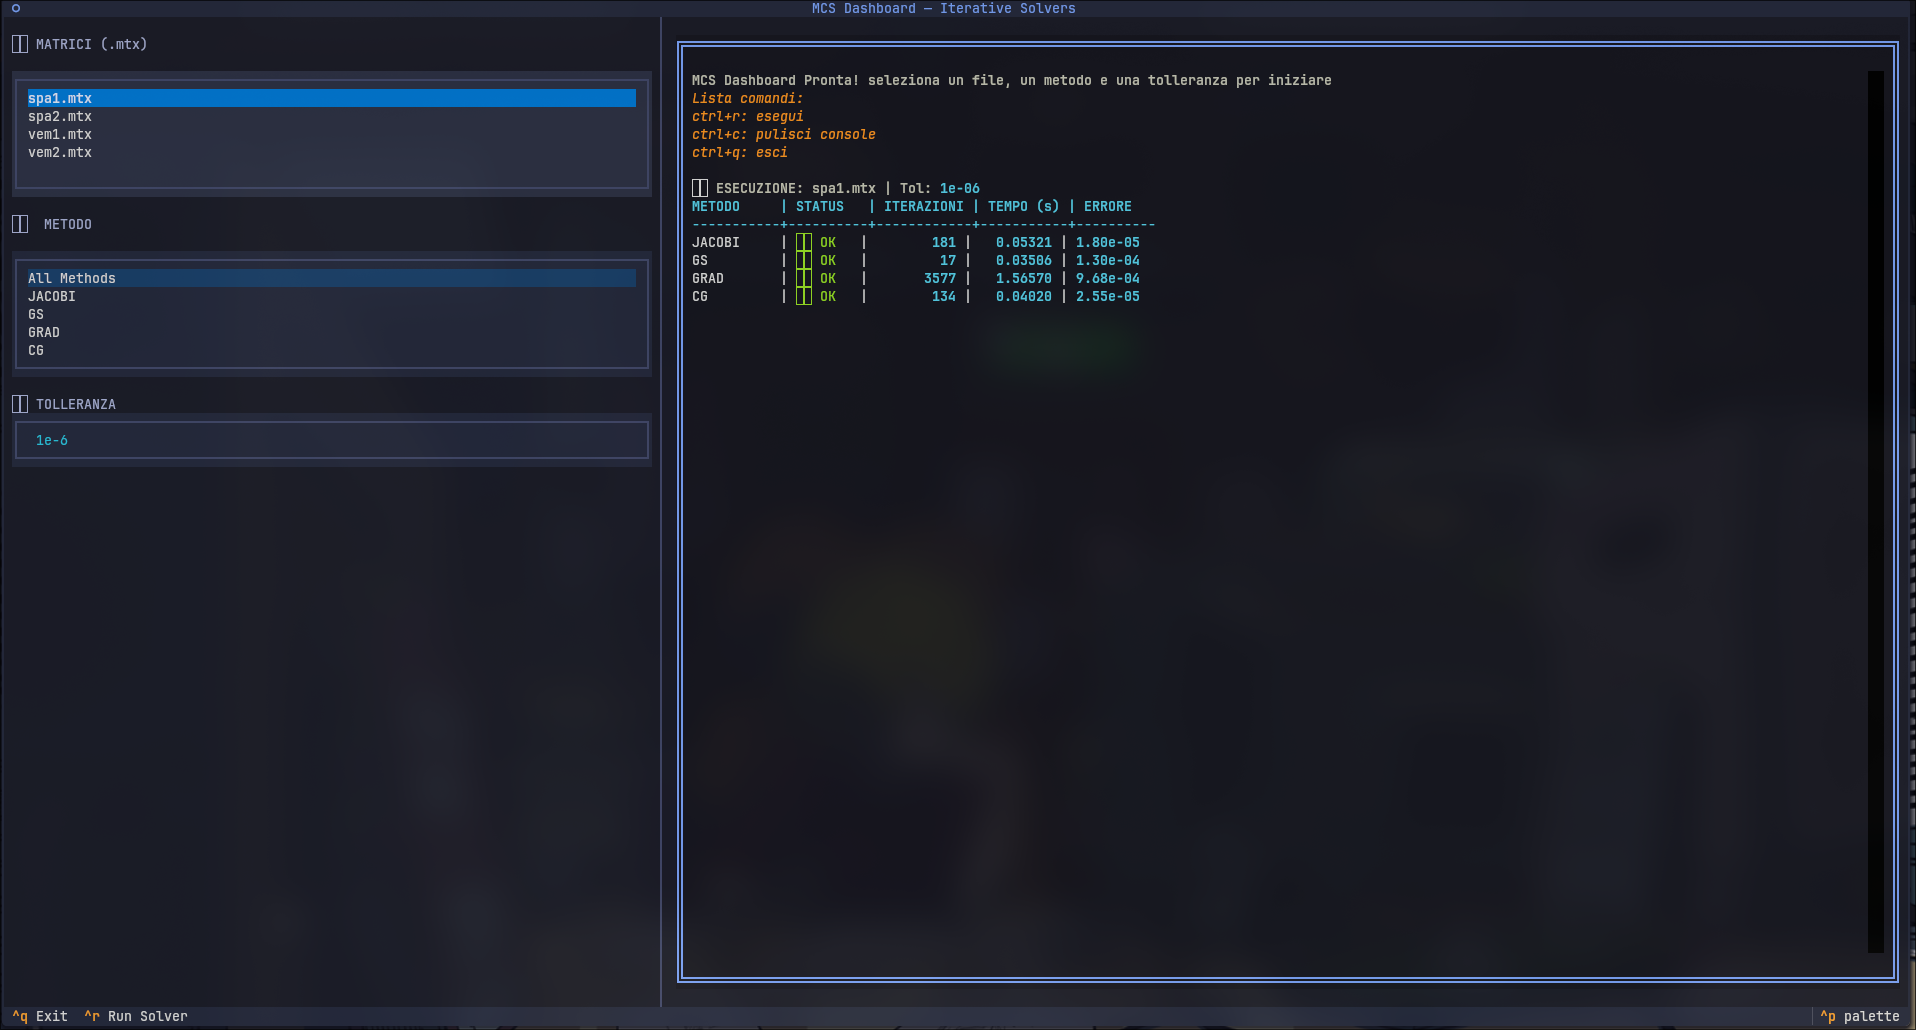
\includegraphics[width=0.9\textwidth]{images/TUI.png}
    \caption{Interfaggia Grafica da Terminale TUI.}
    \label{fig:analysis_spa1}
\end{figure}




% ==============================================================================
\section{Matrici di test}
% ==============================================================================
Il dataset fornito comprende quattro matrici sparse in formato Matrix Market (\texttt{.mtx}):
\begin{itemize}
    \item \texttt{spa1.mtx}, \texttt{spa2.mtx} : matrici di dimensioni relativamente contenute, con struttura a bande e buone proprietà spettrali.
    \item \texttt{vem1.mtx}, \texttt{vem2.mtx} : matrici provenienti da discretizzazioni agli elementi virtuali (VEM), di dimensioni maggiori e con spettro più ampio e numero di condizionamento più elevato.
\end{itemize}
Tutte sono simmetriche e definite positive, e presentano un'elevata sparsità . La struttura spettrale influisce direttamente sulla velocità di convergenza di tutti i metodi iterativi, come evidenziato nei risultati sperimentali.

% ==============================================================================
\section{Risultati sperimentali}
% ==============================================================================
Il benchmark è stato eseguito per tolleranze decrescenti:
\begin{equation}
    \text{tol} \in \{10^{-2},\; 10^{-4},\; 10^{-6},\; 10^{-8},\; 10^{-10}\}.
\end{equation}
I grafici generati da \texttt{plotter.py} mostrano chiaramente le prestazioni relative dei quattro solutori. Di seguito vengono riportati e commentati i risultati principali.

\subsection{Confronto complessivo}
I risultati mostrano comportamenti molto diversi a seconda della matrice,
e non esiste un ordinamento fisso tra i metodi valido in tutti i casi.

\begin{itemize}
    \item \textbf{Gradiente Coniugato} è il metodo più robusto: mantiene un
    numero di iterazioni estremamente basso su tutte le matrici e domina
    nettamente su \texttt{vem1} e \texttt{vem2}, dove gli altri metodi
    degradano sensibilmente. È l'unica scelta affidabile al crescere del
    numero di condizionamento.

    \item \textbf{Gauss-Seidel} presenta un comportamento opposto a seconda
    della matrice. Su \texttt{spa1} e \texttt{spa2} è competitivo in termini
    di tempo — su \texttt{spa2} risulta addirittura più veloce del CG — grazie
    al basso costo per iterazione. Su \texttt{vem1} e \texttt{vem2} diventa
    invece il metodo \emph{più lento} in assoluto: pur avendo meno iterazioni
    di Jacobi, il costo della sostituzione in avanti su struttura densa scala
    male con la dimensione, portando a tempi fino a un ordine di grandezza
    superiori agli altri.

    \item \textbf{Jacobi} è stabile e prevedibile: il numero di iterazioni
    cresce linearmente con la tolleranza e il costo per iterazione è basso.
    Su \texttt{vem1} e \texttt{vem2} è più lento di GRAD e CG in iterazioni,
    ma più veloce di GS in tempo grazie alla semplicità dell'aggiornamento.

    \item \textbf{Gradiente (Steepest Descent)} mostra il comportamento più
    anomalo: su \texttt{spa1} e \texttt{spa2} esplode completamente, con
    oltre $10\,000$ iterazioni a tolleranza $10^{-10}$, probabilmente a causa di un forte comportamento 
    a zig zag che lo porta ad oscillare attorno al minimo.
    Su \texttt{vem1} e \texttt{vem2}, nonostante un numero di condizionamento piu alto, si comporta invece in modo simile a
    Jacobi, rimanendo nella stessa fascia di iterazioni e tempi.
\end{itemize}

\subsection{Grafici comparativi}
Le Figure~\ref{fig:analysis_spa1}, \ref{fig:analysis_spa2}, \ref{fig:analysis_vem1}
e \ref{fig:analysis_vem2} mostrano per ciascuna matrice l'evoluzione del tempo
di calcolo e del numero di iterazioni al variare della tolleranza.

Su \texttt{spa1} (Figura~\ref{fig:analysis_spa1}) il Gradiente esplode in
iterazioni mentre gli altri tre metodi rimangono comparabili in tempo; il CG
è il più veloce ma il margine su GS e Jacobi è contenuto.

Su \texttt{spa2} (Figura~\ref{fig:analysis_spa2}) il quadro è analogo, con la
differenza che GS risulta il più veloce in tempo grazie al basso numero di
iterazioni combinato con un costo per iterazione ancora gestibile sulla
dimensione di questa matrice.

Su \texttt{vem1} (Figura~\ref{fig:analysis_vem1}) il CG è nettamente separato
dagli altri (circa $1$--$3$ ms contro decine o centinaia), mentre GS diventa
il \emph{peggiore} in tempo nonostante abbia meno iterazioni di Jacobi,
evidenziando come il costo della sostituzione in avanti diventi dominante.

Su \texttt{vem2} (Figura~\ref{fig:analysis_vem2}) il distacco di CG si
accentua ulteriormente e GS raggiunge tempi dell'ordine dei $10\,000$ ms,
peggio di tutti gli altri metodi. Jacobi e GRAD si comportano in modo simile
sia in iterazioni che in tempo.

\begin{figure}[H]
    \centering
    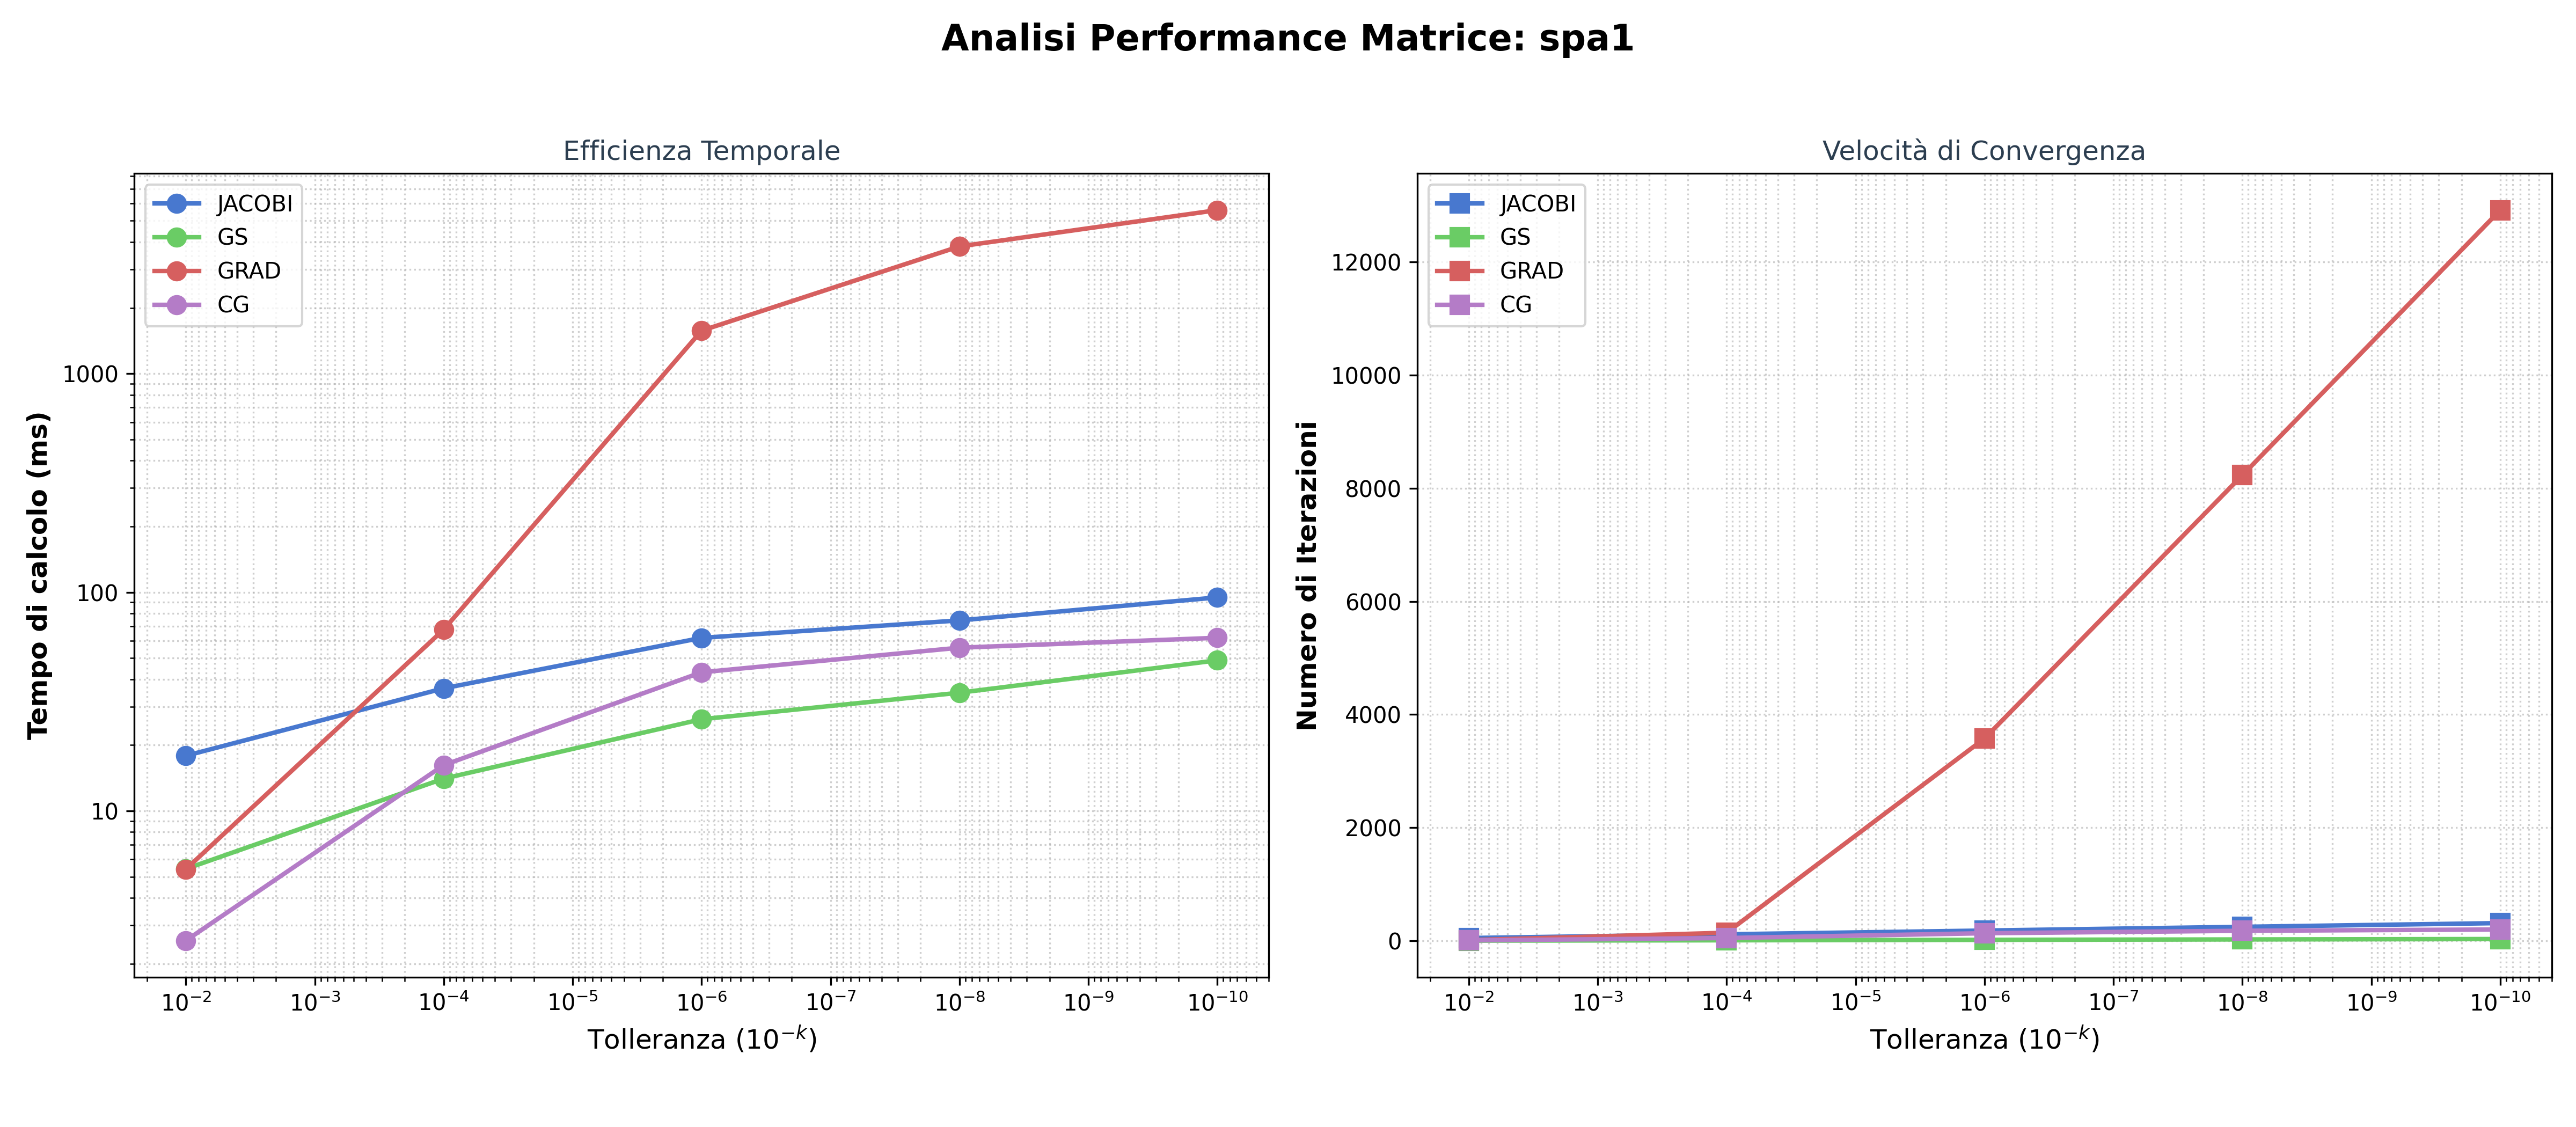
\includegraphics[width=0.9\textwidth]{images/analysis_spa1.png}
    \caption{Matrice SPA1: tempo di calcolo e numero di iterazioni al variare della tolleranza.}
    \label{fig:analysis_spa1}
\end{figure}

\begin{figure}[H]
    \centering
    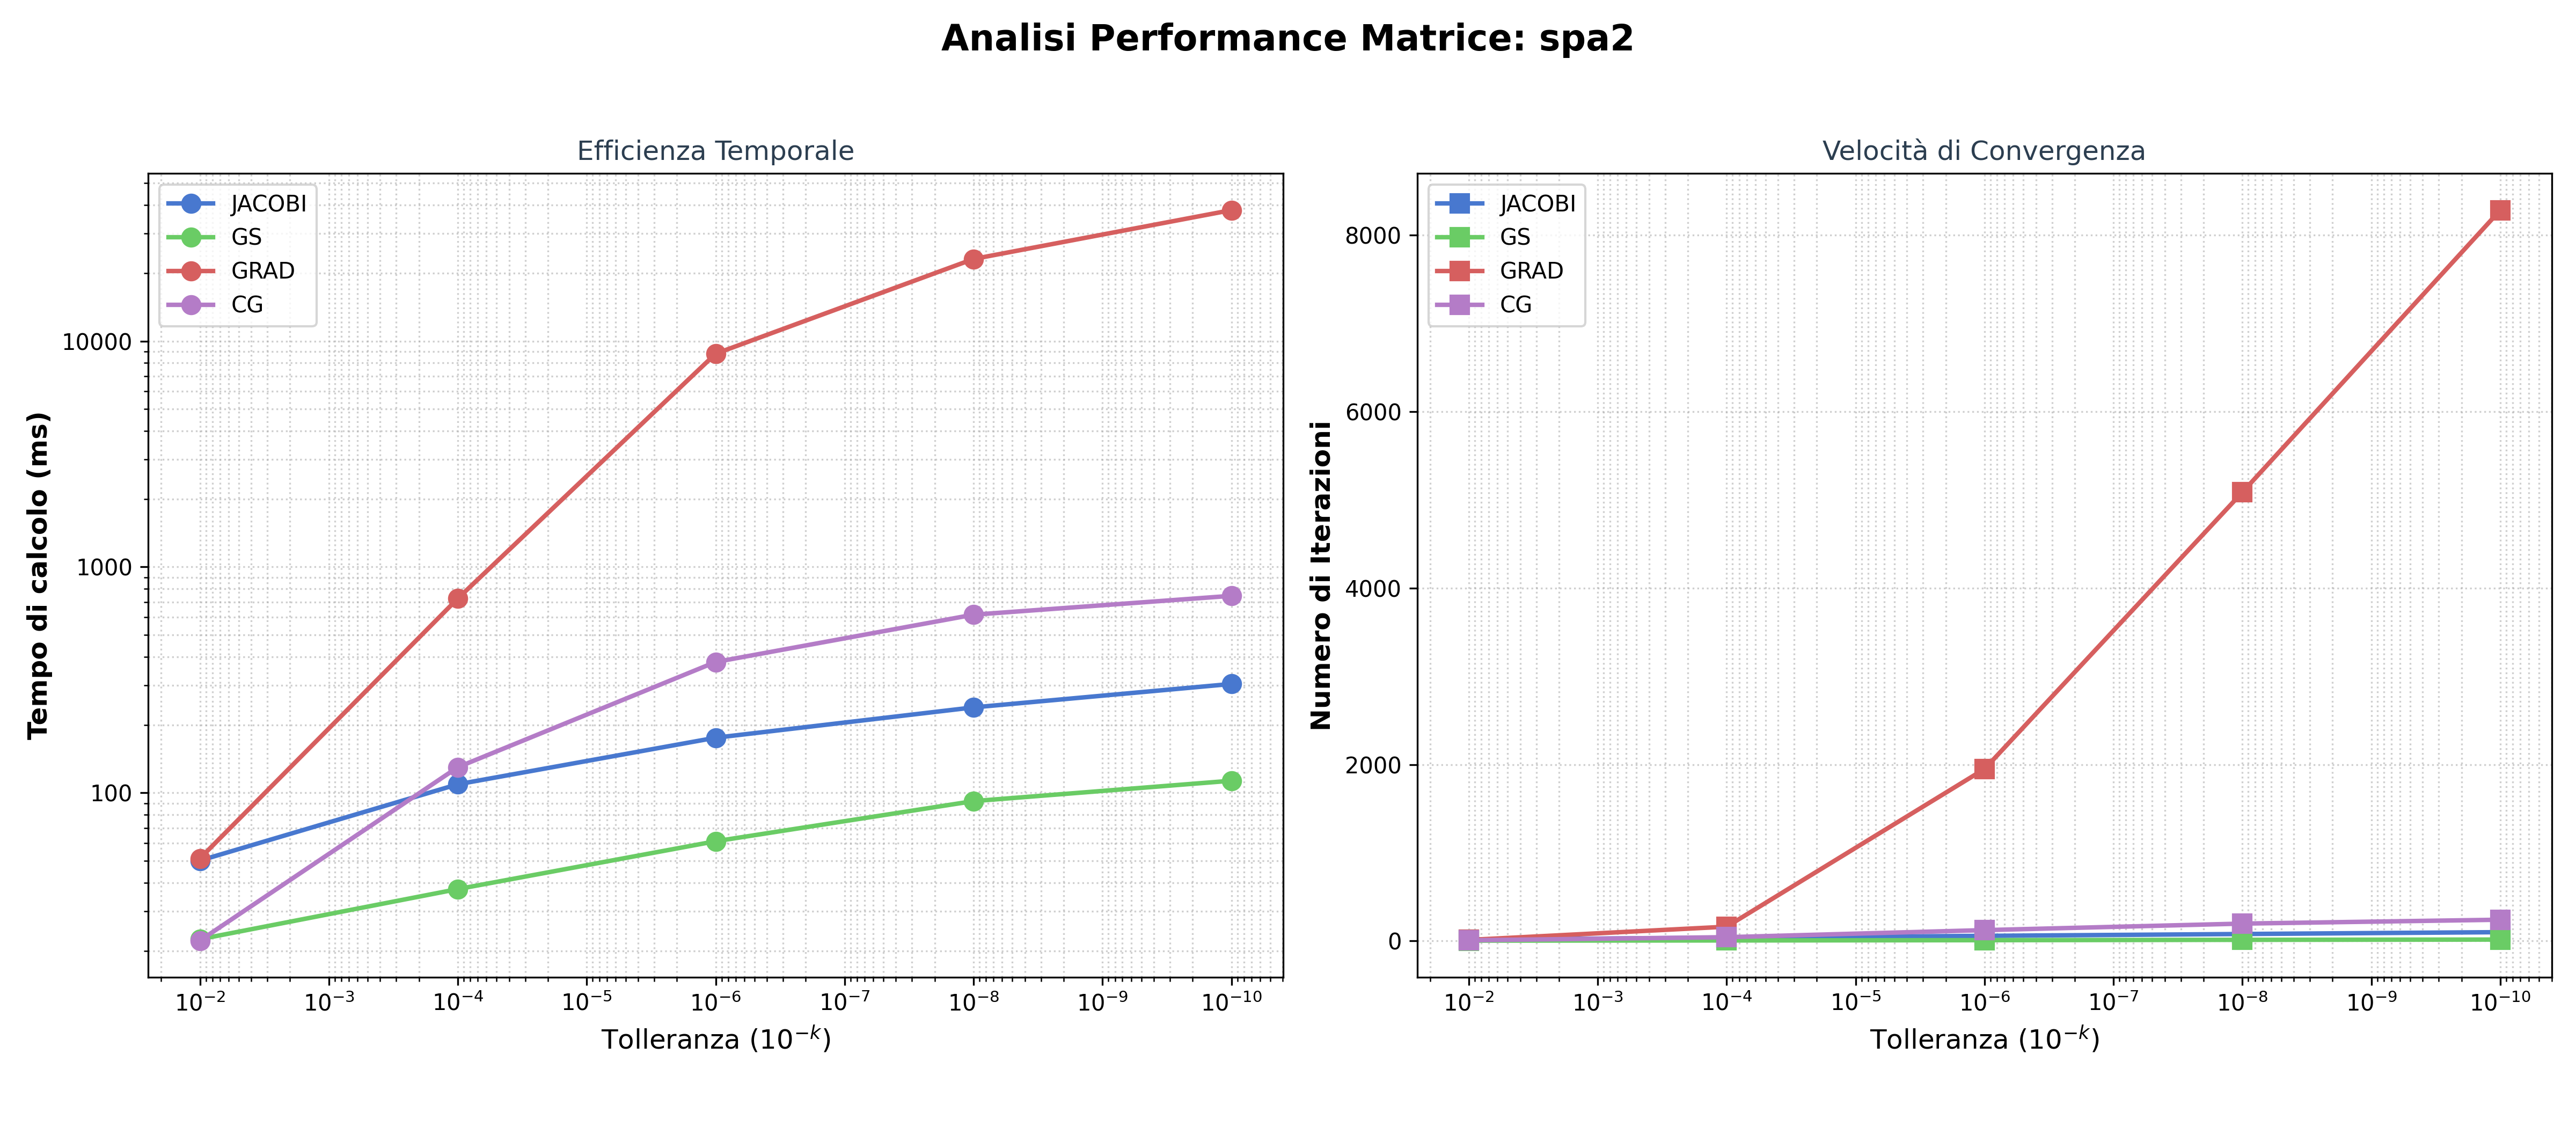
\includegraphics[width=0.9\textwidth]{images/analysis_spa2.png}
    \caption{Matrice SPA2: tempo di calcolo e numero di iterazioni al variare della tolleranza.}
    \label{fig:analysis_spa2}
\end{figure}

\begin{figure}[H]
    \centering
    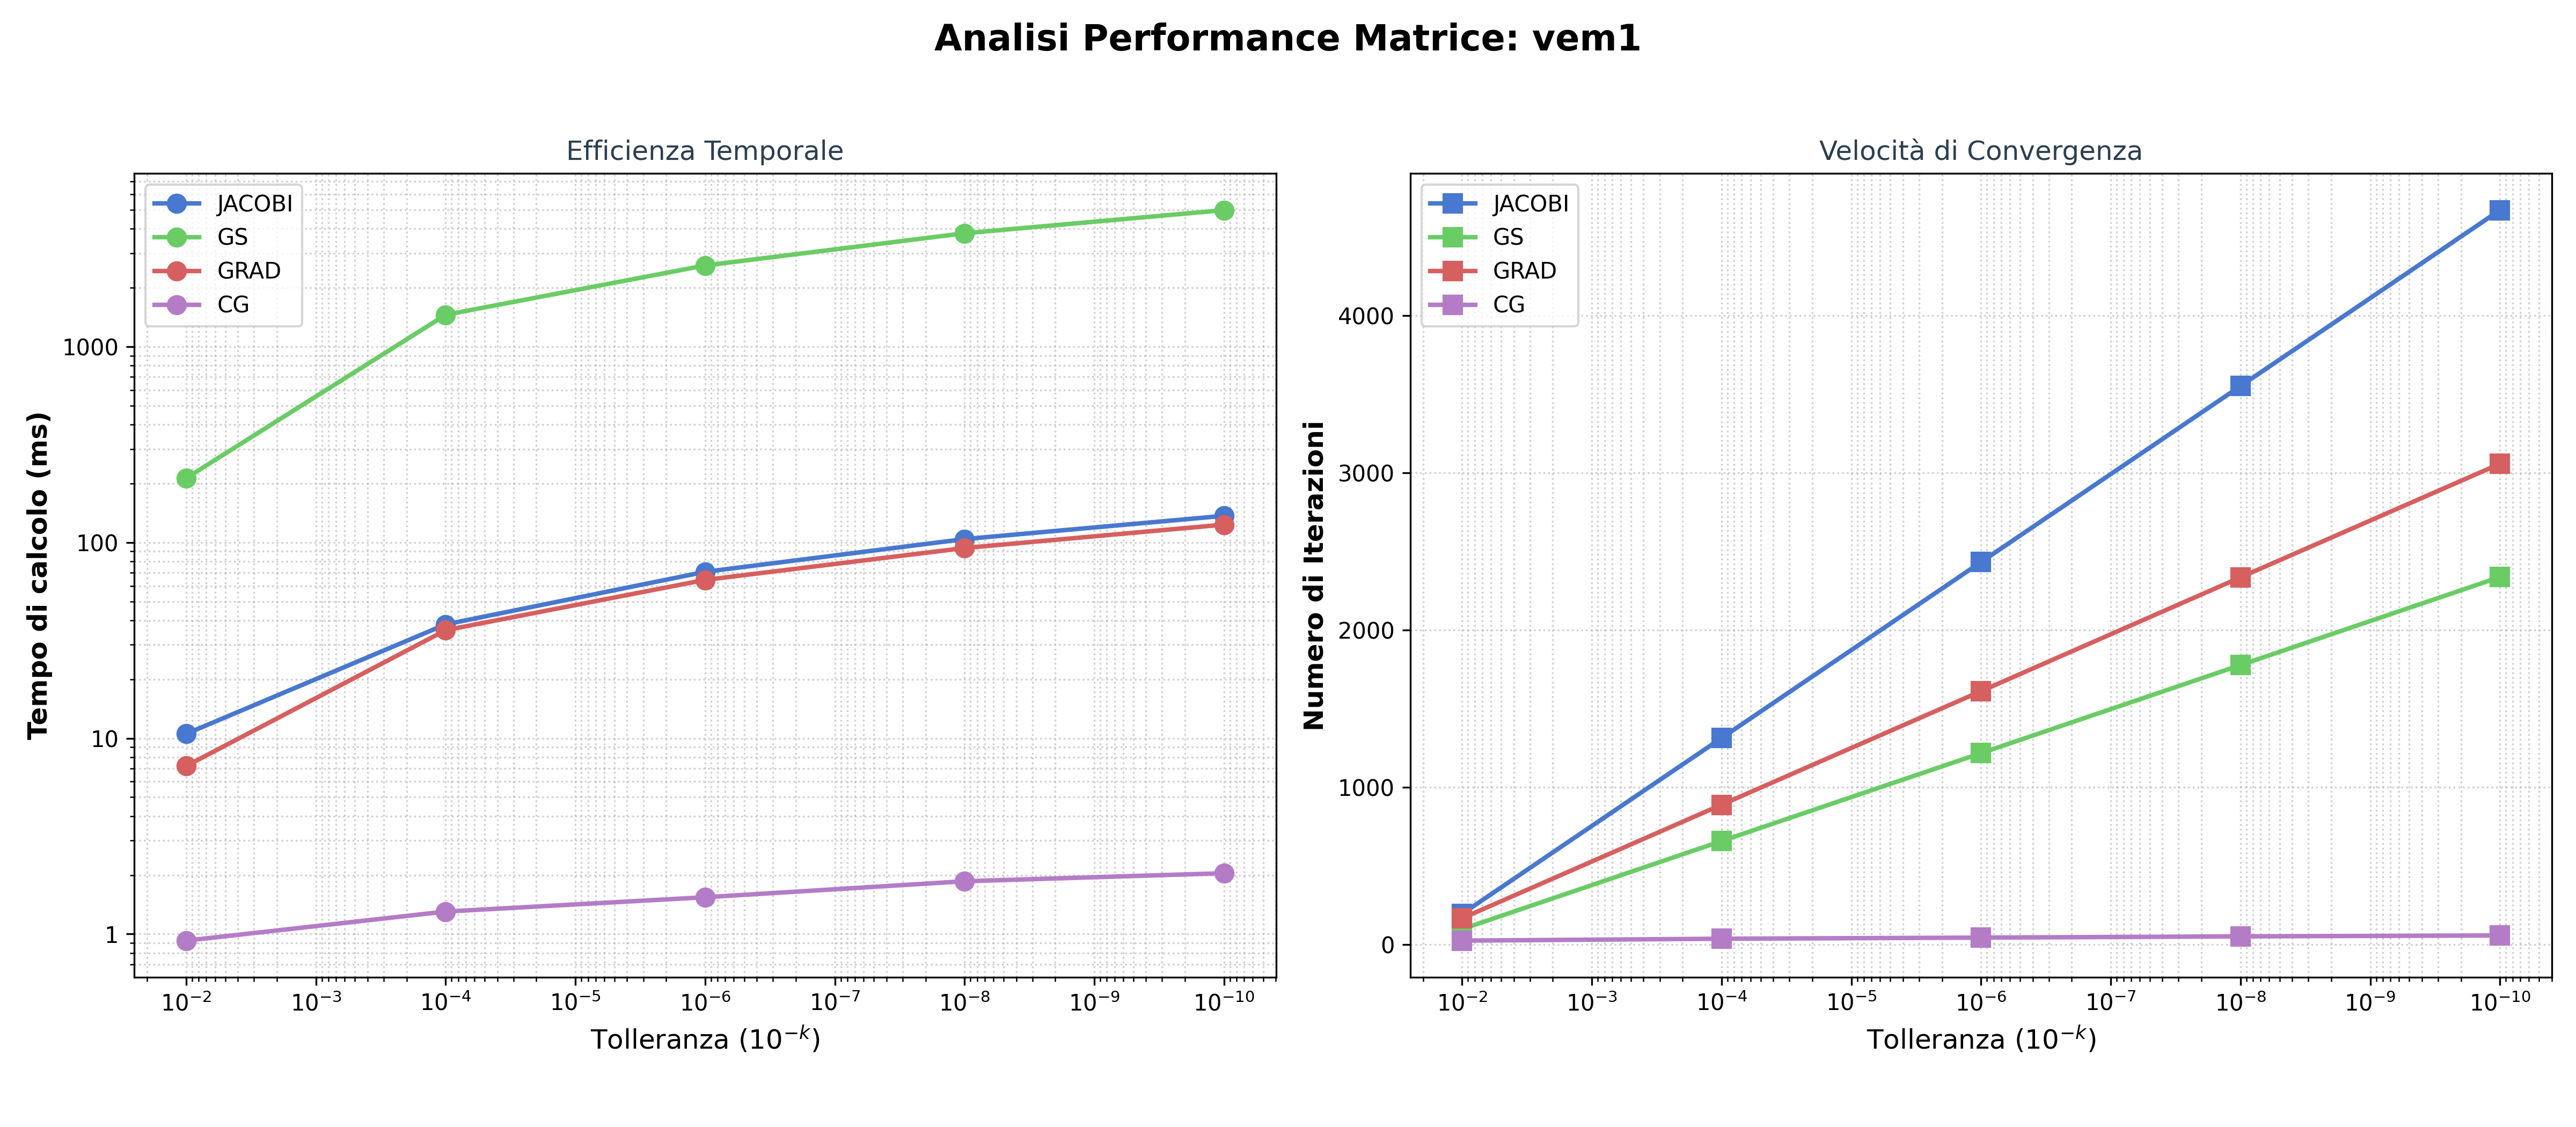
\includegraphics[width=0.9\textwidth]{images/analysis_vem1.png}
    \caption{Matrice VEM1: tempo di calcolo e numero di iterazioni al variare della tolleranza.}
    \label{fig:analysis_vem1}
\end{figure}

\begin{figure}[H]
    \centering
    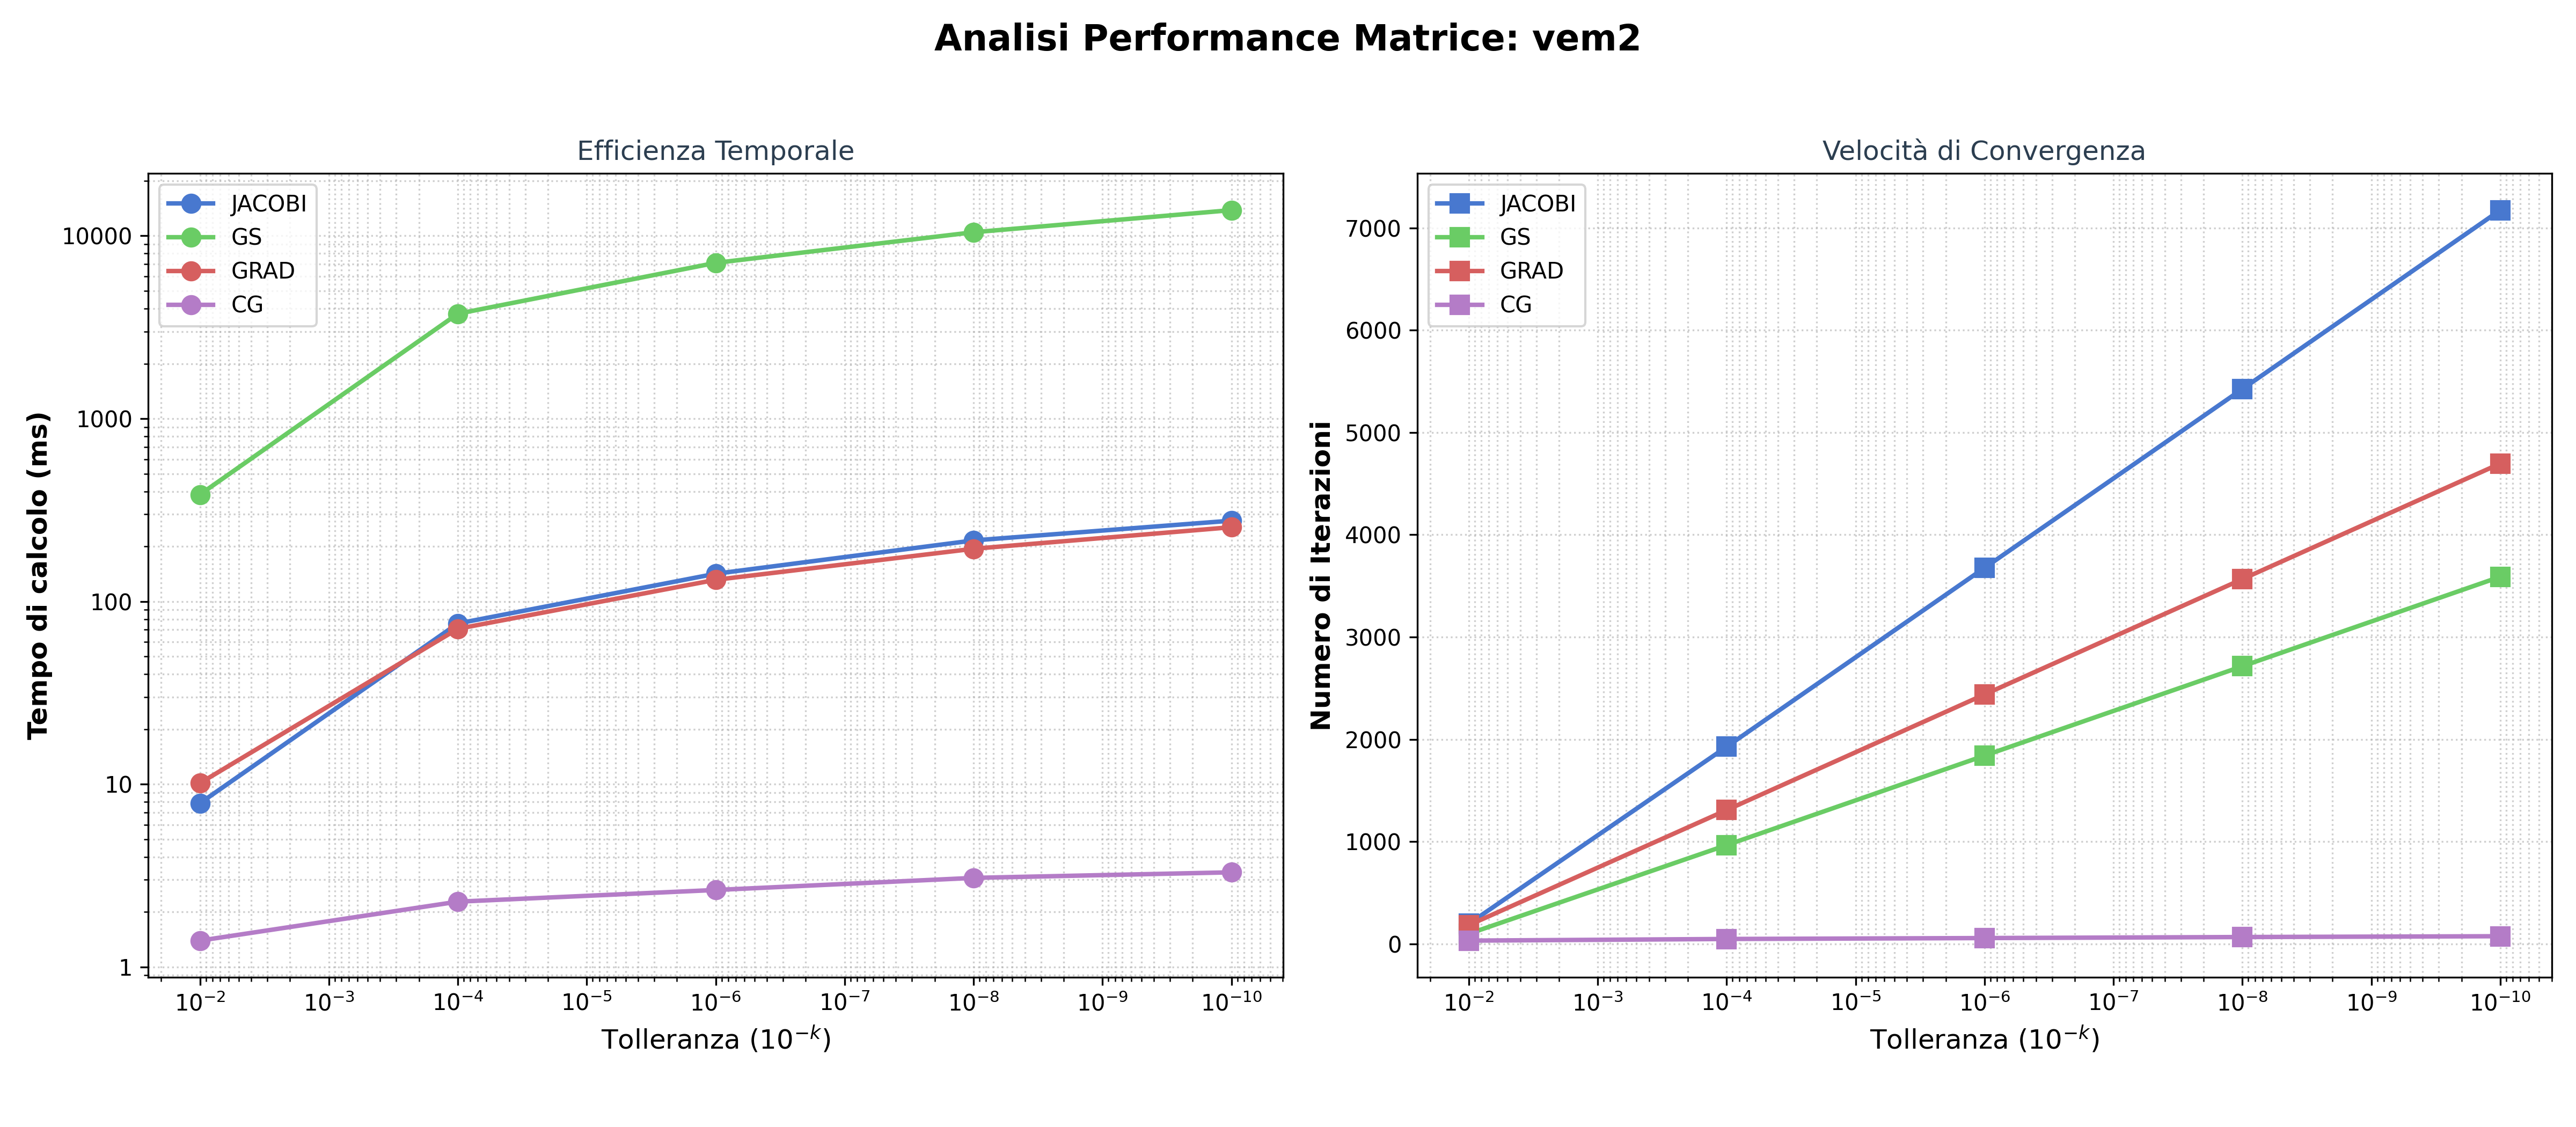
\includegraphics[width=0.9\textwidth]{images/analysis_vem2.png}
    \caption{Matrice VEM2: tempo di calcolo e numero di iterazioni al variare della tolleranza.}
    \label{fig:analysis_vem2}
\end{figure}

% ==============================================================================
\section{Conclusioni}
% ==============================================================================
Il progetto ha raggiunto l'obiettivo di implementare e confrontare quattro solutori iterativi per sistemi lineari SPD, affiancati da un'interfaccia a riga di comando e da una TUI moderna. L'architettura modulare del codice e lo script di benchmark hanno permesso un'analisi sistematica delle prestazioni al variare di matrice e tolleranza.

I risultati confermano la superiorità del Gradiente Coniugato, che unisce velocità di convergenza e stabilità numerica, risultando la scelta ottimale per sistemi SPD di grandi dimensioni. I metodi di Jacobi e Gauss-Seidel, pur semplici da implementare, richiedono molte più iterazioni; Gauss-Seidel è generalmente preferibile a Jacobi, ma l'implementazione naive su formato denso ne limita la scalabilità. Il metodo del Gradiente, pur convergente, soffre del fenomeno di zig-zag su problemi mal condizionati.


L'attività ha permesso di approfondire non solo gli aspetti teorici dei metodi iterativi, ma anche di vedere in modo pratico come la scelta del solutore non
sia mai indifferente: matrici con struttura e condizionamento diversi
premiano metodi diversi, e affidarsi a un unico algoritmo senza analizzarne
le proprietà può portare a prestazioni peggiori, come dimostrato da
Gauss-Seidel su \texttt{vem2} o dal Gradiente su \texttt{spa1}.

\appendix
\section{Istruzioni per l'esecuzione}
\label{app:run}

\subsection{Requisiti}
\begin{lstlisting}[language=bash]
pip install -r requirements.txt
\end{lstlisting}
Il file \texttt{requirements.txt} include NumPy, SciPy, Matplotlib, Pandas e Textual.

\subsection{Esecuzione di un singolo test (CLI)}
\begin{lstlisting}[language=bash]
python main.py -f Data/spa1.mtx -t 1e-6 -s 4
\end{lstlisting}

\subsection{Interfaccia TUI}
\begin{lstlisting}[language=bash]
python app.py
\end{lstlisting}
Utilizzare \texttt{Ctrl+R} per eseguire, \texttt{Ctrl+C} per pulire la console, \texttt{Ctrl+Q} per uscire.

\subsection{Benchmark completo}
\begin{lstlisting}[language=bash]
python benchmark.py
python plotter.py
\end{lstlisting}
I risultati numerici vengono salvati in \texttt{Data/benchmark\_results.csv} e i grafici nella cartella \texttt{Data/Plot/}.

\end{document}